\documentclass[11pt,titlepage,a4paper,twocolumn]{article}
\usepackage{graphicx} % Required for inserting images
\usepackage[a4paper, total={6.5 in, 9 in}]{geometry} %this will adjust the height and width of thr height of the text, total={width, height}
\usepackage{amsmath}
\usepackage{times}
\pagestyle{plain}% this will add page nuneber under
\graphicspath{ {images/} }
\usepackage{array,url,kantlipsum}
\newcommand{\Mark}[1]{\textsuperscript{#1}}
\usepackage[font=footnotesize]{caption}
\usepackage{float}
\usepackage{xcolor}
\usepackage{titlesec}
\titlespacing*{\subsubsection}{0pt}{0.1\baselineskip}{0.2\baselineskip}
\usepackage{gensymb}
\titlespacing*{\subsection}{0pt}{0.1\baselineskip}{0.2\baselineskip}


\begin{document}

\title{University of Toronto \\ PHY 180 Pendulum Lab Report}
\author{None}
\date{December 6th, 2023}
\maketitle

\twocolumn[
  \begin{@twocolumnfalse}
    \maketitle
    {\fontsize{22pt}{30pt}\selectfont \textbf{Homemade Pendulum Analysis: Testing of the Credibility of Mathematical Models}}
    % You can put more single column content here
    \vspace{1cm} % Adjust this space according to your needs
  \end{@twocolumnfalse}
]

\section{Introduction}
    \hspace{\parindent}\hspace{\parindent} Pendulums find extensive applications in various areas, including pendulum clocks and earthquake seismometers. Their distinctive periodic behavior makes them a commonly employed tool. Physicists have formulated numerous equations to predict various parameters associated with pendulums. This lab aims to employ a homemade pendulum to assess the accuracy of these equations and ascertain the level of precision.

    Part 1 of the lab explores the relationship between the release angle and the period. After conducting 32 trials, the results indicate that the period and release angle are quadratically related, aligning with the power series equation ($T$ is the period, $T_0$ is the average period, $\theta$ is the release angle):
    \begin{equation} 
    T = T_0(1 + B\theta_0^2 + C\theta_0^2 + \ldots) \label{eq:1}
    \end{equation}
    This contradicts the prediction of the period's independence from the release angle. However, when the release angle is less than 0.4 radians, the period falls well within one error bound, revealing that the prediction of independence of the period from the release angle holds true only when the angle is sufficiently small.
    
    Part 2 of the lab addresses the disparity between the counted Q-value (which determines the pendulum's quality, where higher values are better) and the theoretically derived Q-factor. Two equations are employed to find Q. The first equation is used to determine $\tau$ ($\theta$ is the angle, $\theta_0$ is the initial angle, $\tau$ is the constant, $t$ is the time, $T$ is the period, and $\phi_0$ is the initial phase shift):
    \begin{equation} 
    \theta(t) = \theta_0 e^{-t/\tau}\cos(2\pi \frac{t}{T}+\phi_0)
    \end{equation}
    Subsequently, the $\tau$-value is utilized in the following equation to find Q:
    \begin{equation} 
    Q = \pi \frac{\tau}{T}
    \end{equation}
    The counting method involves tallying the number of periods the pendulum swings before it reaches 20\% of its original angle, corresponding to $\frac{Q}{2}$. The results demonstrate that both the counted and theoretically obtained values fall within their uncertainty ranges, confirming the validity of the two mathematical equations. Moreover, smaller release angles yield higher Q-values, as evident in several other trials.
    
    Part 3 of the lab investigates whether the equation 
    \begin{equation}
    T = KL^n
    \end{equation}
    and the prediction of \(K = 2\) and \(n = 0.5\)
    \begin{equation}
    T = 2\sqrt{L}
    \end{equation}
    accurately describe the relationship between the pendulum's length and period. The experimental values for \(K\) and \(n\) are obtained using the log-log plot:
    \begin{equation}
    \log(T) = n\log(L) + \log(K)
    \end{equation}
    The results suggest that both the mathematical model and prediction are correct (experimental \(K\)-value is 2.01 and experimental \(n\)-value is 0.488).
    
    Lastly, part 4 of the lab discusses the relationship between the Q-factor and the length of the pendulum. From the experiment, it is determined that the Q-factor will decrease as the length increases, fitting the following linear model:
    \begin{equation}
    Q = KL + b
    \end{equation}

    The inaccuracies in some mathematical models may be caused by various real-life factors, such as energy loss due to torsion, air resistance, bending of the string, insufficient data collection methods, and other minor physical factors.


\section{Method and Procedure}
    \subsection{The setup of the pendulum}
        {\hspace{\parindent}\hspace{\parindent}The pendulum setup includes a 0.300 m cotton string, a 20-gram weight, adhesive, a protractor, contrasting black and white background papers, and a Xiaomi 13 Ultra phone. Cotton string is chosen as the mass is negligible compared to the weight; two strings were used to form a basket with the top portion of wire located at the weight’s center, minimizing asymmetry and preventing rotation during oscillation. Weight is used because the uniform mass distribution design reduces rotation risks. The protractor with the origin glued near the wire’s end is used to aid angle observation. Black and white papers are used to enhance OpenCV tracking ability by increasing contrast. The phone is mounted on a suitcase, and aligned parallel with the protractor for optimal data collection, preventing asymmetry. This careful assembly minimizes error sources, ensuring accurate and reliable data during experiments.
        }
        \begin{figure}[H]
        \centering
        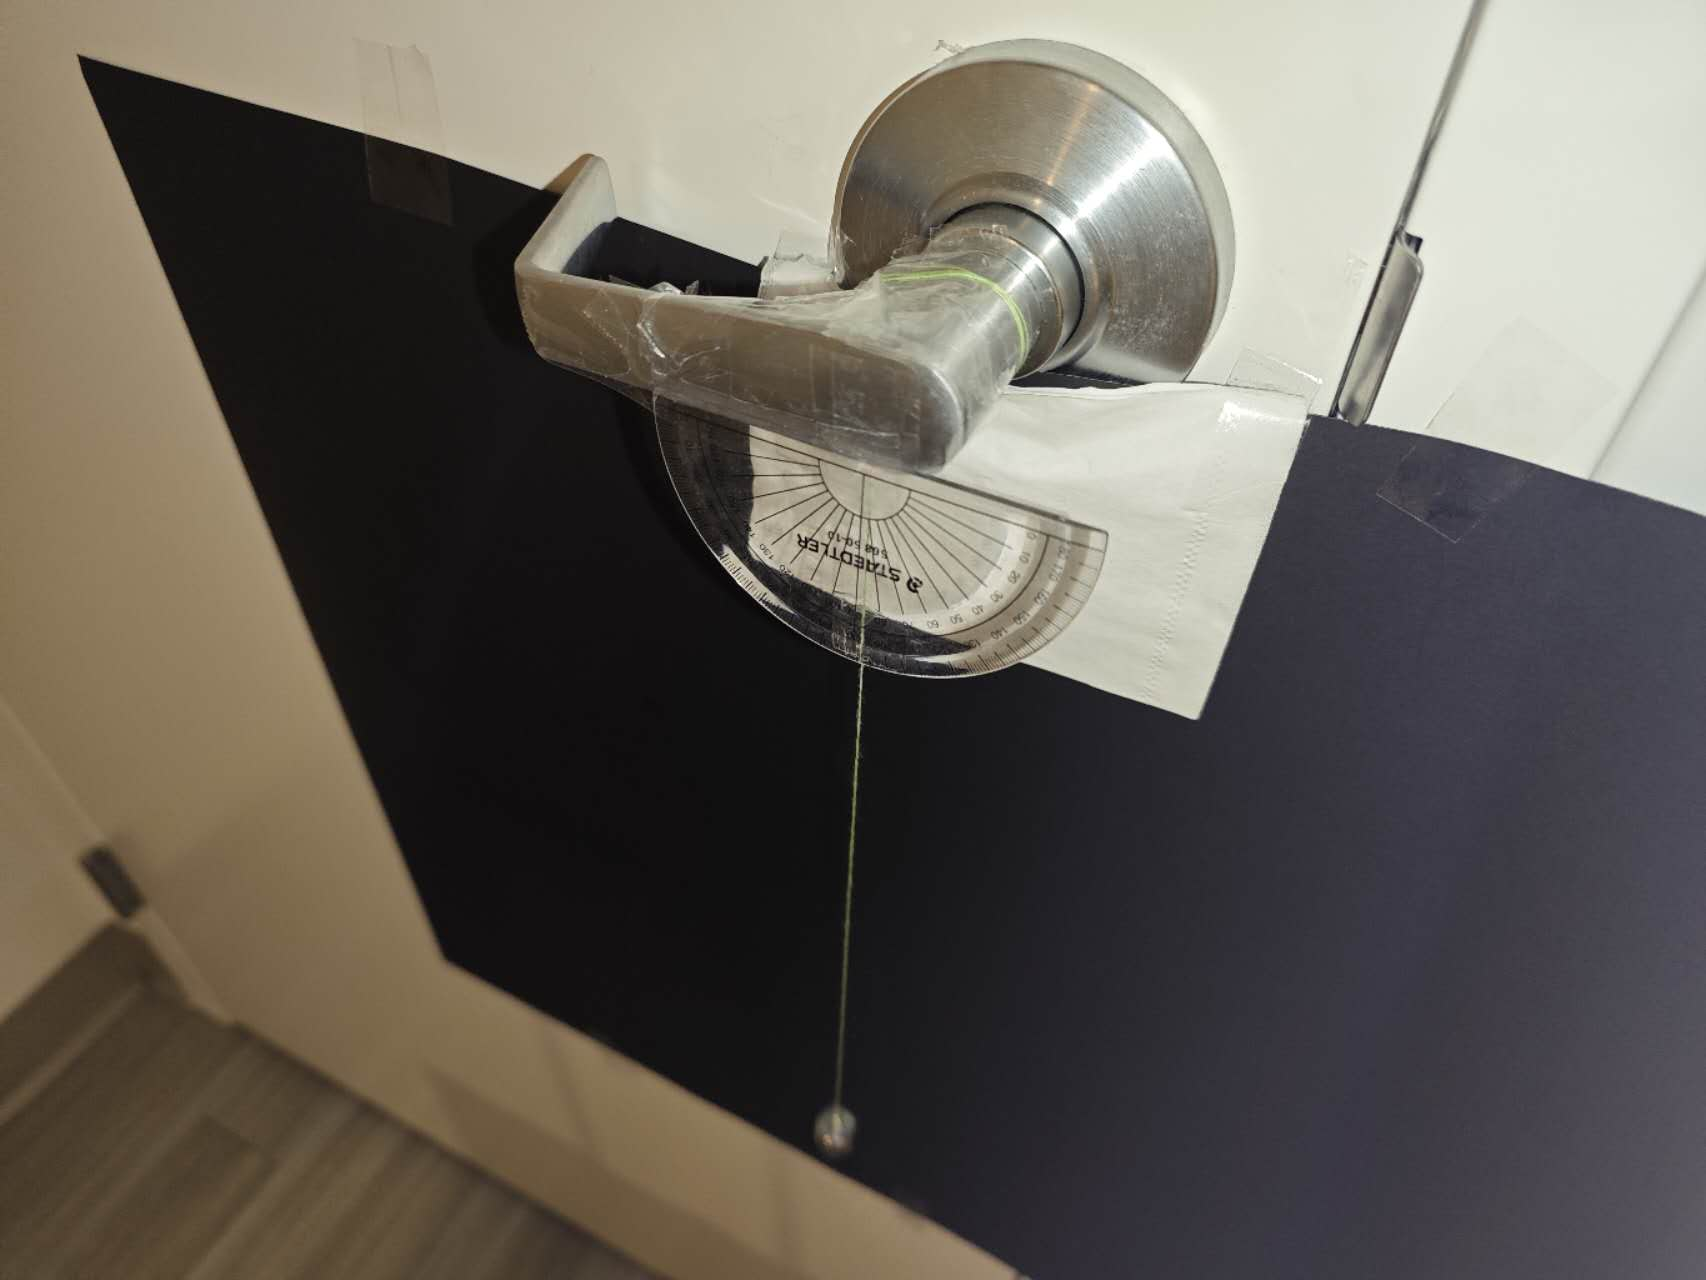
\includegraphics[width=6cm]{setup 1.jpg}
        \captionsetup{labelformat=empty}
        \caption{\textbf{Figure 2.2:} This figure shows the basic overview of the pendulum's setup}
        \end{figure}

        % Do not color the following
    In the second experiment, the original setup was kept because of the small B-value, $B = -1.86\times10^{-4}  \pm 7\times10^{-4} \frac{s}{radians}$ that can be claimed as experimentally zero and a Q-factor over 150, ultimately proving the small asymmetry and the high-quality build. However, due to the varying length, a difference in the result is inevitable.
    
    \begin{figure}
        \centering
        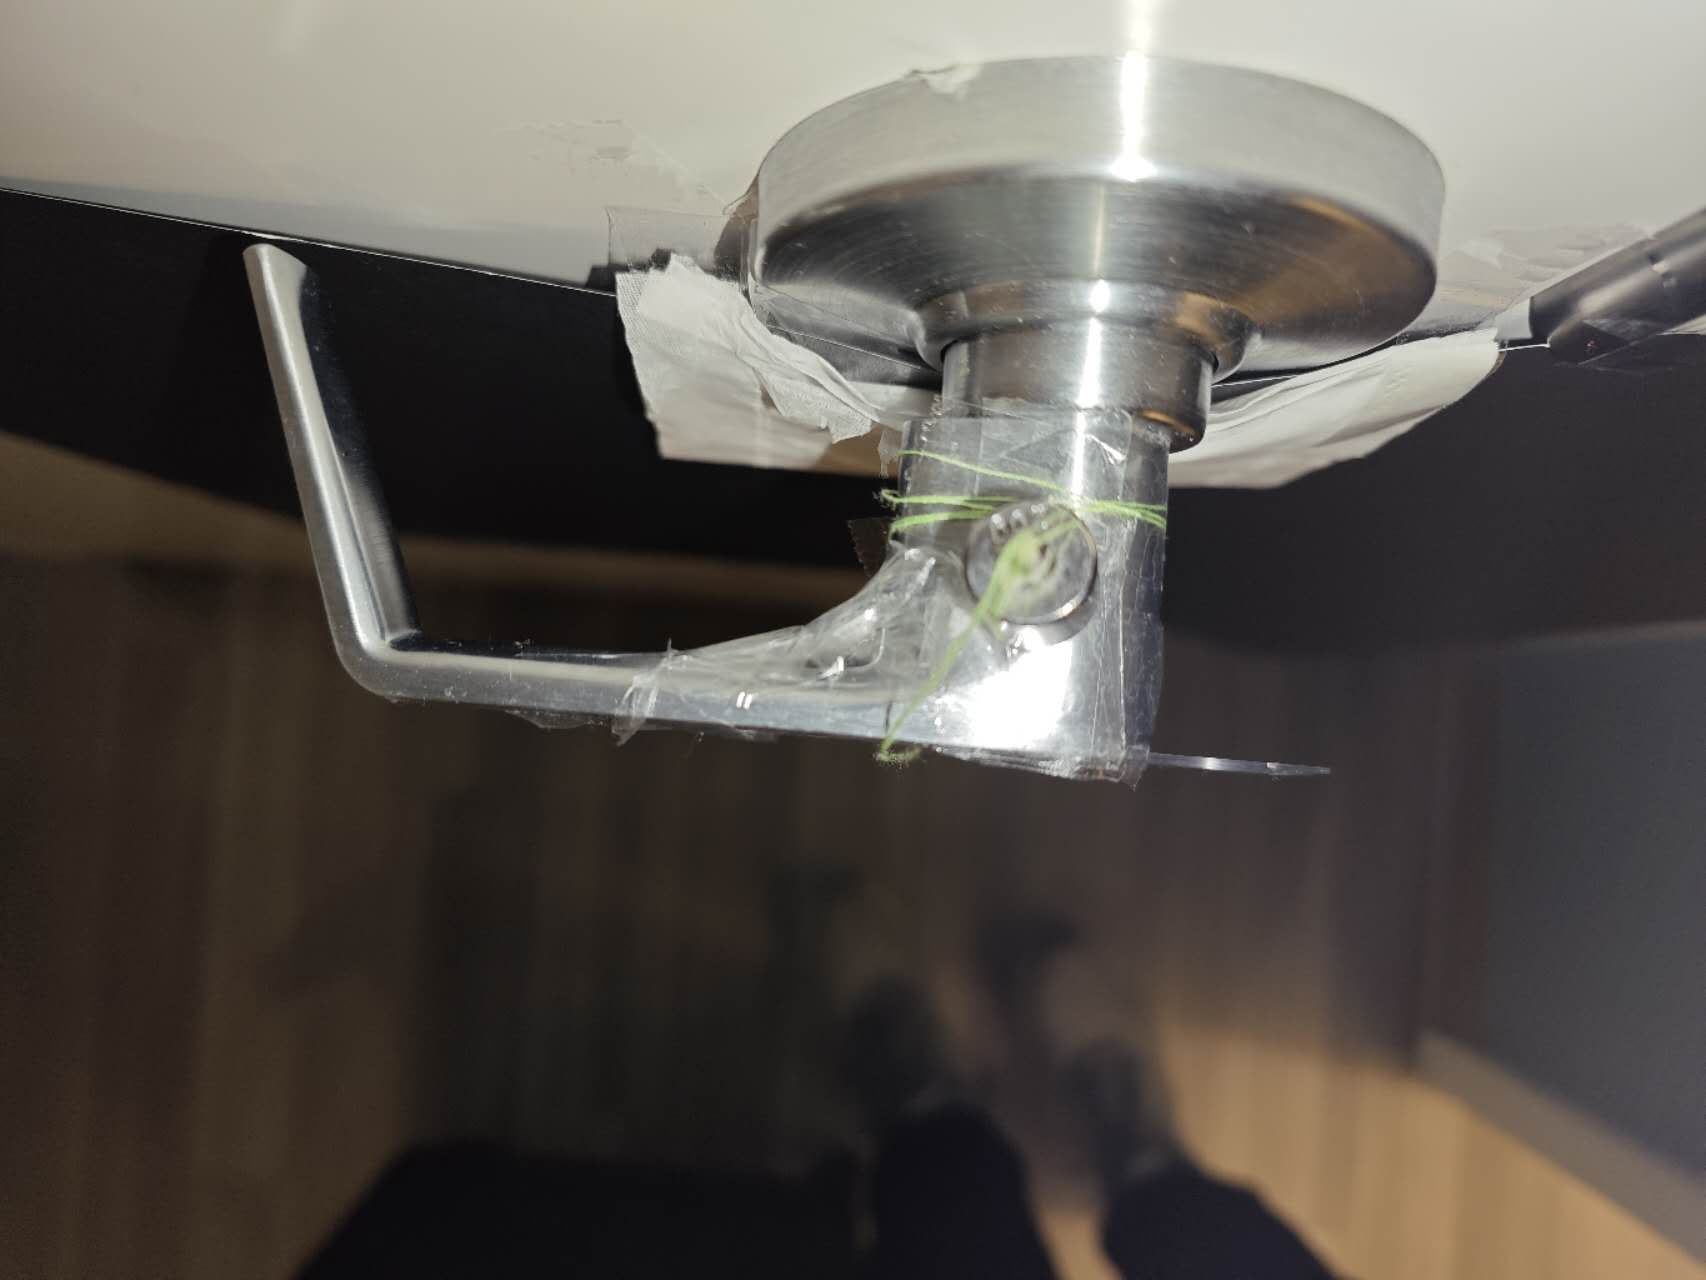
\includegraphics[width=6cm]{setup2.jpg}
        \caption*{\textbf{Figure 2.1:} This figure shows how the weight is tightened}
        \label{fig:enter-label}
    \end{figure}
    \subsection{The Procedure to Measure the Relationship between Release Angle and Period}
        \hspace{\parindent}\hspace{\parindent}{32 videos were recorded with the weight released from -1.39/-80\degree to 1.39 radians/80\degree (2 trials per angle) with 0.175-radian/10\degree differences and 30-35 seconds duration under 4K60FPS. Videos were imported into Davinci Resolve 18.5[3] to count the time the weight used to complete 10 cycles (i.e., time needed to come to the original position). The average cycle times from two videos for each angle were calculated and then divided by 10 to obtain the average period for each release angle, mitigating the effect of other physical factors.
    \subsection{The Procedure to Measure the Q value}
        \hspace{\parindent}\hspace{\parindent}A 253-second video was recorded at 4K60FPS, with the weight released at a 0.524 radians/30\degree angle. OpenCV[2] was utilized for tracking and analyzing the footage, producing a CSV file with frame-vs-angle data. 13 values from this file were used to calculate $\tau$ in Python and to derive the Q-factor. Experimentally, the Q-factor was determined by counting the oscillations until the maximum angle reduced to 20\% of its original value and then multiplying by 2.
    \subsection{The Procedure to Measure Period and Q-factor with Varying Length}
        \hspace{\parindent}\hspace{\parindent}The part of the string that was tightened to the handle was taken off and labeled with 8 red points with a common difference of 10 cm. The distance of the point ranges from 20 cm to 90 cm from the location where the string is tight to the handle. Videos were taken from a length of 90 cm to 20 cm, with the string being pulled back 10 cm and re-tightened each time. A total of 16 videos each with a duration of 6 minutes were taken (2 videos for each length) with the same camera setting from above. The period and Q-factor of each length were obtained using the same procedure from 2.2 and 2.3 with the release angle at 0.524 radians/30$\degree$.


\section{Result and Data Analysis}
    \subsection{The Relationship Between Release Angle and Period}
        \subsubsection{Analysis}
            \hspace{\parindent}\hspace{\parindent}Values from figure 3.1 below were plotted via a Python script, with $T_0$, $B$, and $C$ as parameters in the power series $T = T_0(1 + B\theta_0 + C\theta_0^2 + .....)$. The parameters are $T_0 = 1.13  \pm 1\times10^{-3} $ s $, B = -1.86\times10^{-4}  \pm 7\times10^{-4}$ $\frac{s}{radians}, C = 5.83\times10^{-2} \pm 1\times10^{-3} \frac{s}{radians^2}$. Figure 3.1 indicates a quadratic relationship between the pendulum's period and release angle as the trend line lies in all uncertainty range, suggesting inaccurate predictions for B and C, while other coefficients’ predictions(should be zero) were accurate. However, B can be claimed as experimentally zero as it is smaller than the uncertainty. The $T_0$-value estimates the pendulum’s period, with B's marginal value indicating the pendulum is a well-designed, minimally asymmetrical pendulum since B affects the vertex’s distance from the origin. A non-zero C-value, resulting from factors like handle vibration and wire torsion, suggests a quadratic relationship. However, it is worth noting for angles smaller than 0.4 radians, the period's variation is within one uncertainty range, which suggests release angles under 0.4 radians approximately have a constant period.
            \begin{figure}[H]
                \centering
                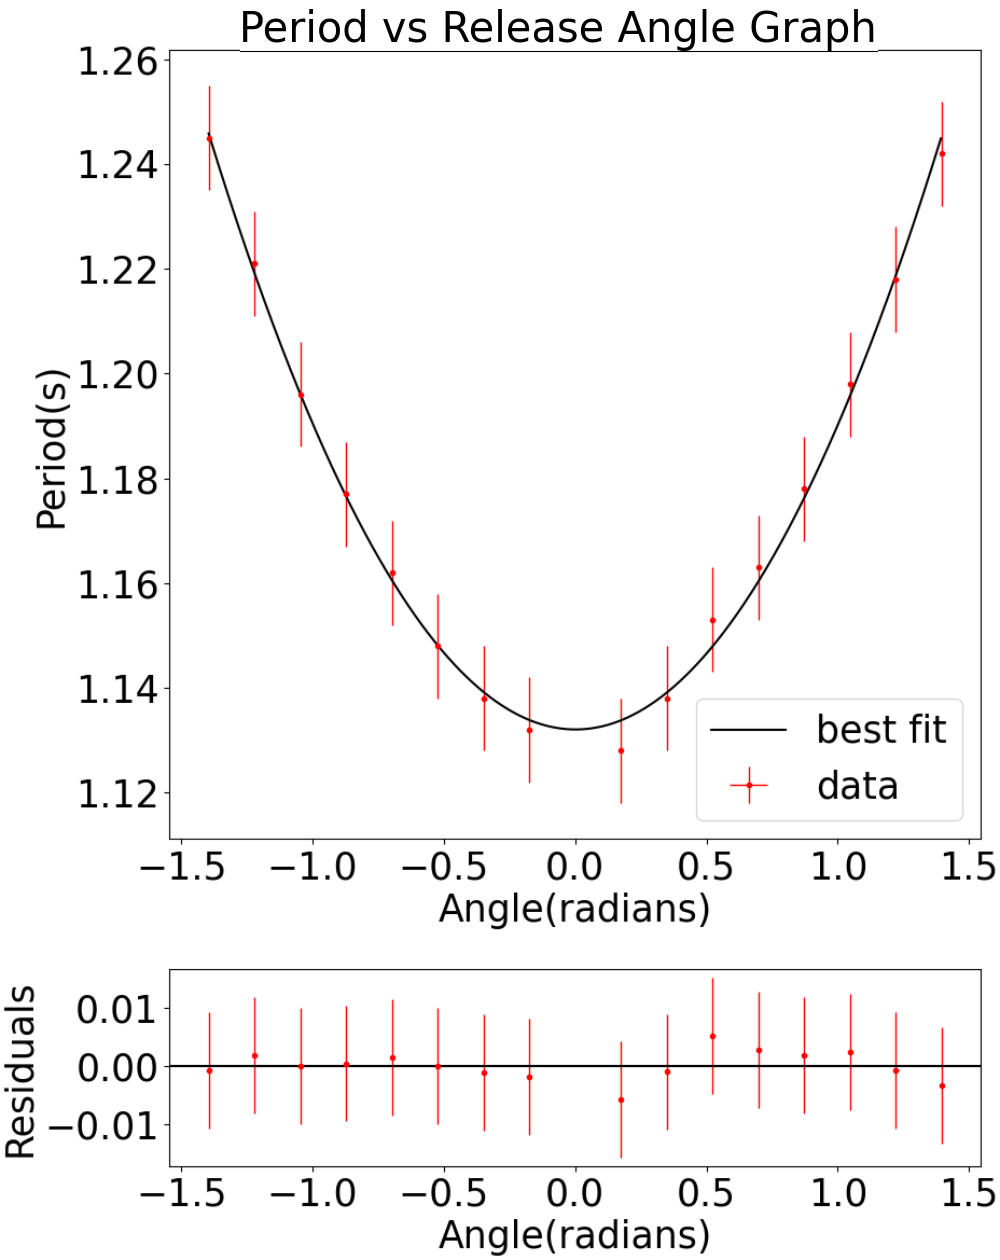
\includegraphics[width=8cm]{3.1.png}
                \caption*{\textbf{Figure 3.1:} Period vs Release angle graph obtained from the experimental data. It reveals period is in quadratic relation with release angle. It also shows the pendulum is well designed as the function is very symmetrical.}
                \label{fig:enter-label}
            \end{figure}
        \subsubsection{Uncertainties}
        \hspace{\parindent}\hspace{\parindent}The protractor's most precise measurement is 0.018 radians/1\degree, resulting in an uncertainty of $\pm 0.009$ radians/0.5\degree (Uncertainty Source 1). OpenCV[2] utilizes color contrast for tracking, but the lighting and video blur prevent it from accurately track the weight's center introducing angle uncertainty. The analysis determined an average deviation of approximately 3 pixels from the center; using basic trigonometry, $\theta = \tan^{-1}\frac{y}{x}$, the tracking uncertainty is estimated at 0.002 radians (Uncertainty Source 2). Videos were recorded at 60FPS (frames per second), or $\frac{1}{60} = 0.01667s$, which creates difficulty to find exact time for 10 oscillations. This time uncertainty doubles to 0.03 seconds as it is derived from two videos (Uncertainty Source 3). Additionally, the pendulum's amplitude changes after 10 oscillations due to resistance and energy loss. Calculations, based on the average difference between starting amplitude and amplitude after 10 oscillations across all trials, resulting in an amplitude decreasing around 10\% (Uncertainty Source 4). Since most error stems from the video recording frame rate (Sources 2 and 3), the greatest source of uncertainty is identified as video recording. Future experiments could benefit from cameras with higher frame rates and enhanced dynamic rate/contrast ratios to minimize blur and improve frame rates.
    \subsection{The Q-factor}
        \subsubsection{Analysis}
            \hspace{\parindent}\hspace{\parindent}Figure 3.2 is generated by substitute the pendulum's every 15 seconds peak over a duration of 253 seconds (excluding the first two data points) into the equation $\theta(t) = \theta_0 e^{-t/\tau}cos(2\pi \frac{t}{T}+\phi_0)$ and set $cos(2\pi \frac{t}{T}+\phi_0) = 1$ (the value of cosine function is 1 at peak),with a release angle of 0.873 radians/50\degree. The parameter is shown to be $\theta_0 = 0.743 \pm 3 \times10^{-2}$ radians and $\tau = 64.3 \pm 2$. It clearly shows the amplitude of the pendulum decreasing exponentially over time via seeing trend line lies in the uncertainty range, which proves the correctness of the mathematical model. The amplitude decreases rapidly immediately after release, suggesting that a larger release angle leads to greater energy loss due to factors like friction, torsion force in the wire, 3D rotation, and wire bending. Consequently, $\tau$ and the Q-factor are most accurately calculated with smaller release angles, such as those below 0.25 radians/14\degree. This fact is further proven by Figure 5.2 in the appendix, which displays the exponential model including the first two data pairs. The error bar and best-fit curve with these data are less accurate than the above graph, mainly due to the first two data pairs acting as outliers. Using the $\tau$ value of $64.3 \pm 2$ and equation $Q=\pi\frac{\tau}{T}$, the theoretical Q-factor is approximately $173 \pm 7$. Using the counting method, the pendulum was released at 0.524 radians/30\degree on two rounds, and the number of oscillations needed to reduce its amplitude to 20\% of its original amplitude (Q/2) was counted. This value was found to be 85 $\pm 3$. By multiplying this value by 2, the Q-factor was determined to be 170 $\pm 6$ using the counting method. Since the Q-factors obtained are within the uncertainties of each other, they can be considered experimentally equal.
                \begin{figure}[H]
                    \centering
                    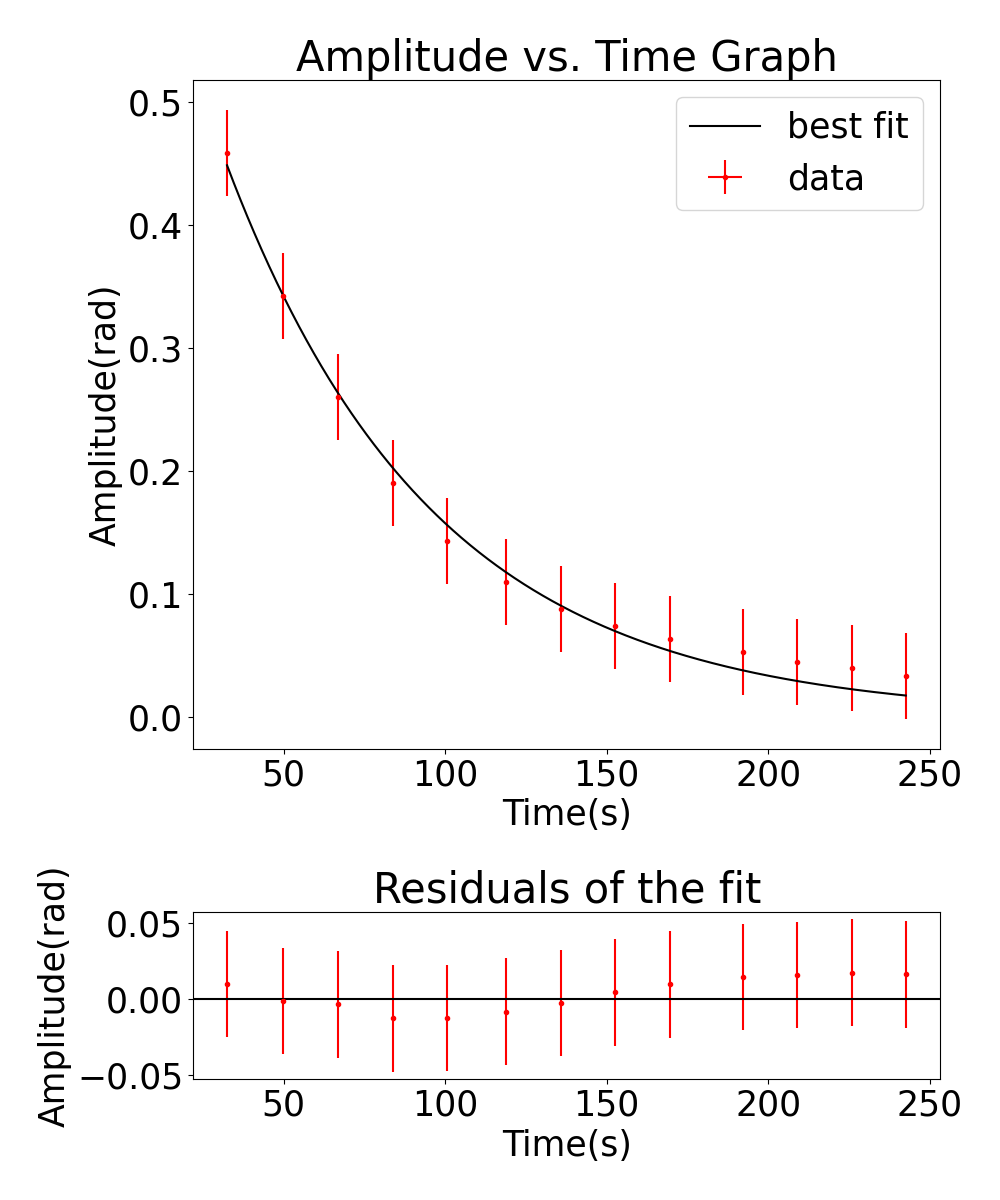
\includegraphics[width=8cm]{3.2.png}
                    \caption*{\textbf{Figure 3.2:} Amplitude vs angle graph obtained from  experimental result. It clearly shows the angle of the pendulum will decrease exponentially as time goes.}
                \end{figure}
            

        \subsubsection{Uncertainties}
            \hspace{\parindent}\hspace{\parindent}Due to imprecision in the protractor, it is challenging to precisely determine when the pendulum reaches 20\% of its original angle, as the angle appears similar for the last three cycles. Therefore, the uncertainty of this measurement for Q-factor is $\pm6$ cycles (Uncertainty Source 5). For the Q-factor obtained from the mathematical equation $\pi \frac{\tau}{T}$, its uncertainty is also multiplied by $\frac{\tau}{T}$, calculated to be $\pm7$ (Uncertainty Source 6). Upon calculation, the largest uncertainty in this part is the 4\% uncertainty from the Python script, which is from the amplitude measured from the video. Therefore, a higher frame rate and dynamic rate camera can be used to record video to decrease such errors in the future.\\
            \textcolor{red}{*}Note that Uncertainty Sources 1, 2, 3, and 4 also affect this part measurement/calculation.}

        
    \subsection{Period vs Length}
        \subsubsection{Analysis/uncertainties}
            \hspace{\parindent}\hspace{\parindent}The values from Figure 3.3 were obtained by changing the length of the pendulum from 0.2 m to 0.9 m and were fitted into the power function $T = KL^n$, resulting in $K = 2.01 \pm 0.01\frac{s}{m^{0.5}}$ and $n = 0.491 \pm 0.01$. The $R^2$ value is 0.988 and the curve of best fit lies within the uncertainty, which indicates that both the mathematical model and the prediction for the parameters are fairly accurate. 
            \begin{figure}[H]
                \centering
                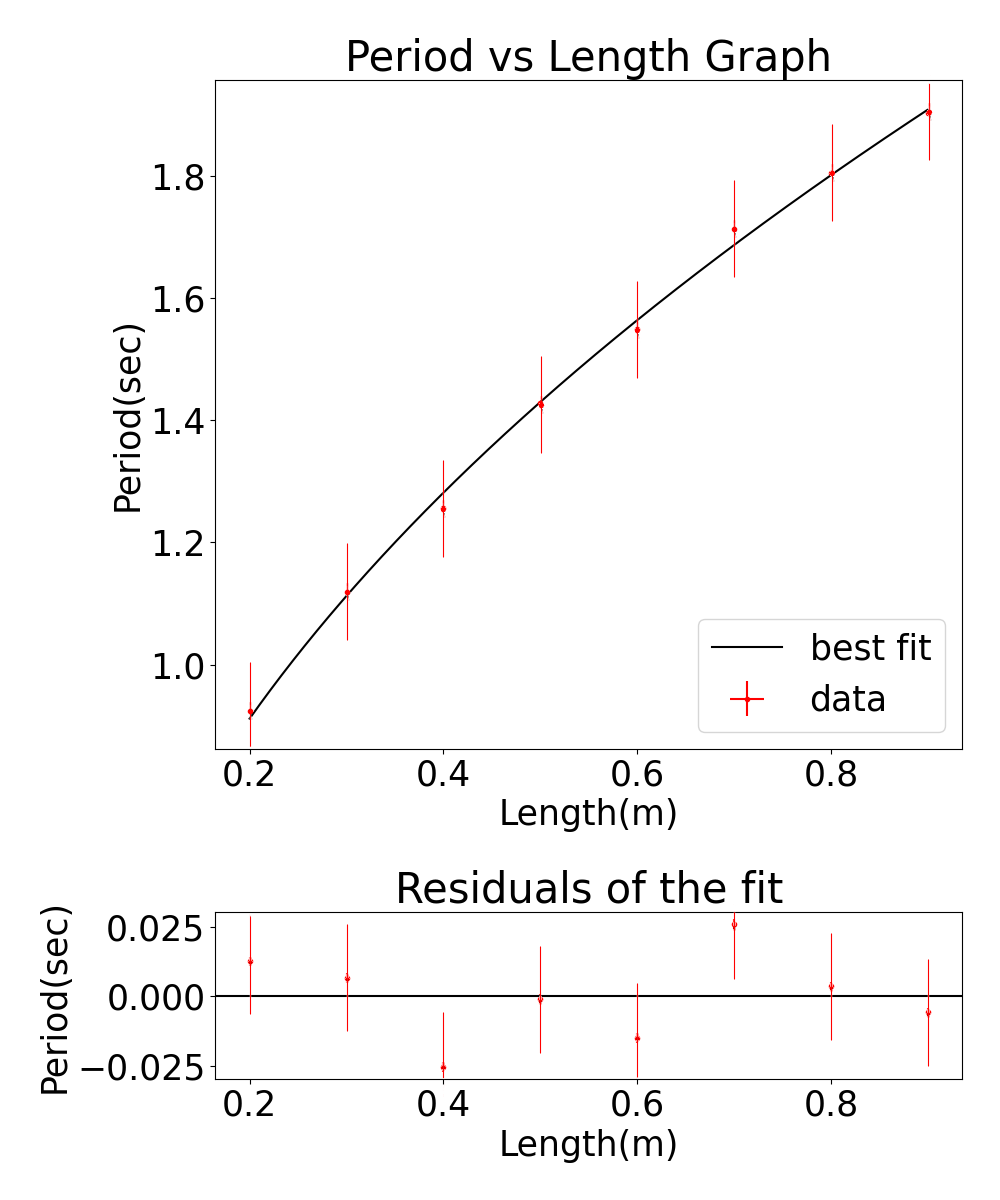
\includegraphics[width=8cm]{3.3.1.png}
                \caption*{\textbf{Figure 3.3:} Length vs. period graph obtained from experimental results. It clearly shows that the period of the pendulum has a power/square root relationship with its length.}
            \end{figure}
    
            \begin{figure}[H]
                \centering
                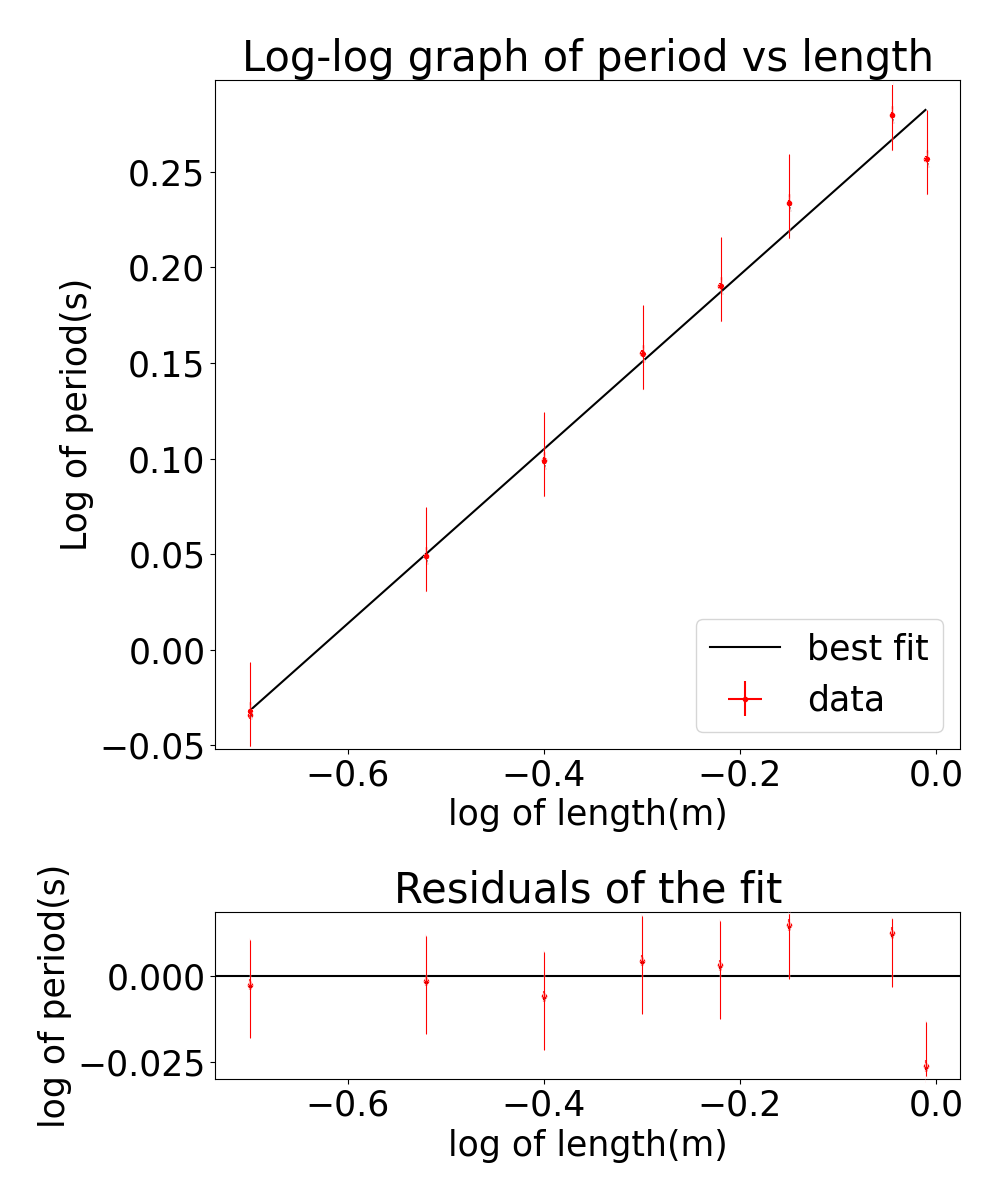
\includegraphics[width=8cm]{3.3.2.png}
                \caption*{\textbf{Figure 3.4:} Log length vs. log period graph obtained from experimental results. It shows a clearer relationship, where increasing length leads to an increase in period.}
            \end{figure}
    
            To further support this point, the values are plotted on a log-log graph. The graph, figure 3.4, follows a linear equation with a slope of $m = 0.456 \pm 0.02\frac{s}{m}$ and a y-intercept of $b = 0.287 \pm 0.008s$. This relationship may be attributed to the increase in arc length while the value of gravitational acceleration remains unchanged, leading to an increase in travel time and period.
            
            \textcolor{red}{*}The uncertainties in this lab may be attributed to the inaccurate installation of the pendulum, as each adjustment to the length of the pendulum may cause it to become looser and result in an inability to obtain accurate measurements of the length. This could lead to an average uncertainty of 1 cm or 0.01 m in length. Note that Uncertainty Sources 1, 2, 3, and 4 also affect this part measurement/calculation. As the uncertainties of source 3 is 0.003s, which is greater than any other uncertainties' effect to period, it is concluded to be the greatest source of error.


    \subsection{Q-factor vs. Length}
        \subsubsection{Analysis/Uncertainties}
            \hspace{\parindent}\hspace{\parindent}Figure 3.5 is formed by plotting the Q-factor for each length from 0.2 m to 0.9 m. After several trials with different models, the linear model ($y = mx + b$) was determined to be the most suitable for this situation. The parameter values are $m = -225 \pm 20\frac{1}{m}$ and $b = 507 \pm 10$. This model clearly shows that the Q-factor decreases with the length of the pendulum. The Q-factor determines the quality of the pendulum, and a perfect pendulum will have negligible weight for the connection part. With the increase in mass due to the increased length, the mass will no longer be negligible, directly decreasing the quality, which is the Q-factor. Furthermore, the longer length will also result in greater wind resistance, causing the string to bend easily and lose energy, decreasing the Q-factor and increase uncertainties. Additionally, the fitting parameter is much greater than its uncertainty range and the line of best fit is within the uncertainty, which is $\pm11$. Thus, it can be said that the fitting parameters are clearly not zero, proving the linear dependence of Q-factor on length.
            \begin{figure}[H]
                \centering
                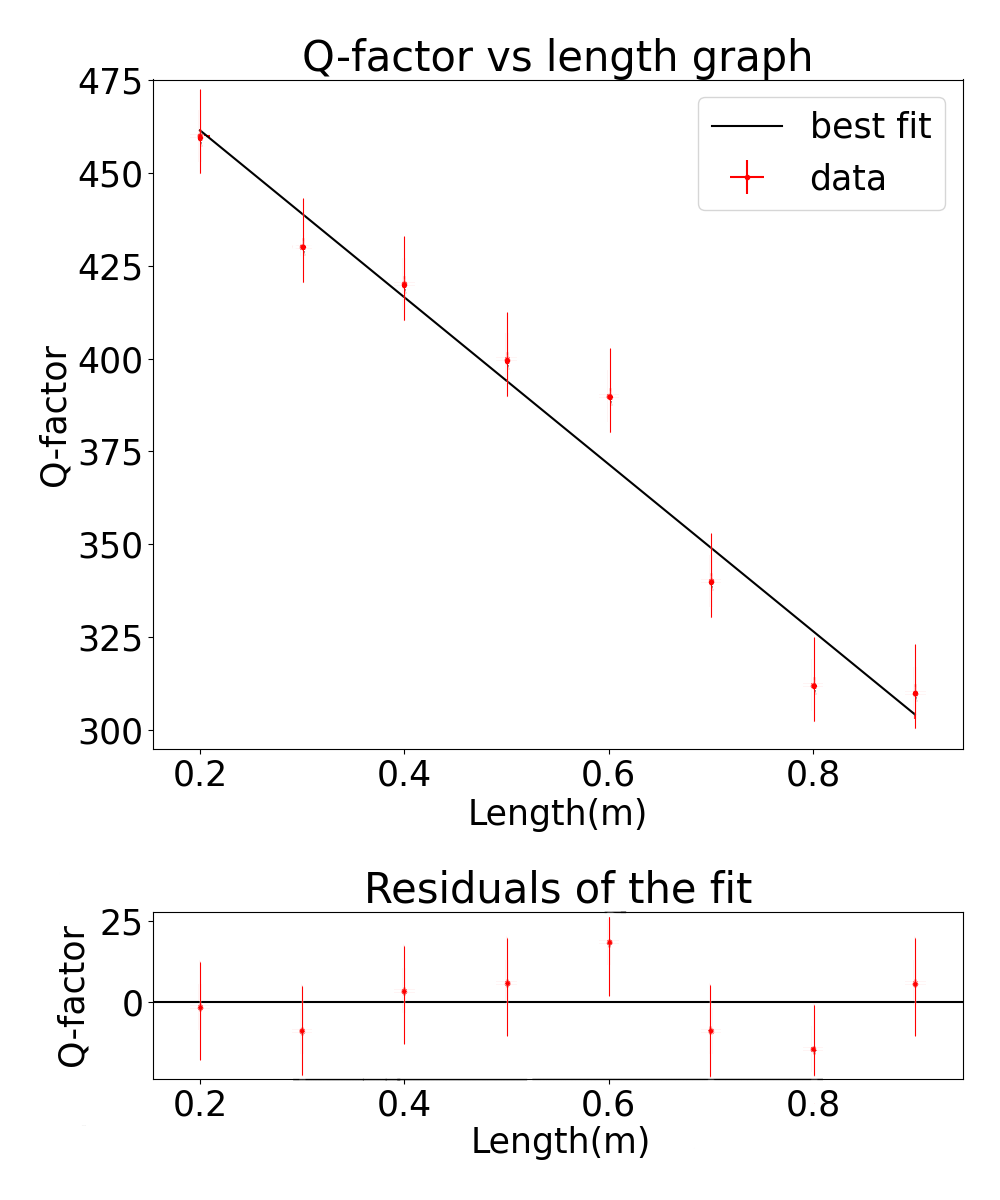
\includegraphics[width=8cm]{3.4.png}
                \caption*{\textbf{Figure 3.5:} Q-factor vs. period graph obtained from experimental results. It shows a clear linear relationship that the increase in pendulum's length will decrease the Q-factor.}
            \end{figure}
    
            The Q-factor values are obtained by counting the number of cycles the pendulum takes to reduce its amplitude to 20\% of its original, which is $\frac{Q}{2}$. Although both methods are applicable, the counting method is better in terms of finding the specific time a specific angle is reached. This could be caused by the small release angle. As mentioned previously, a release angle greater than $40^\circ$ often results in a rapid reduction in amplitude and random motion that creates huge difficulty in finding the Q-factor. However, a small release angle will lead to a much smaller 20\% angle, which creates difficulty for the tracker to determine when the 20\% initial angle is reached. The calculation uncertainties in Python further magnify this problem, causing less precision in finding the Q-factor. With the counting method, it is easier to determine when the 20\% initial angle is reached and fewer calculations are involved, leading to higher precision.

            \textcolor{red}{*}Note that Uncertainty Sources 1, 2, 3, and 4 also affect this part of the measurement/calculation. The greatest uncertainty is again concluded to be source 3, the inaccuracy in video, which is what caused inaccurate measurement in counting for Q-factor.

\section{Conclusion}
    \subsection{Summary}
        \hspace{\parindent}\hspace{\parindent}This homemade pendulum is designed to verify a series of mathematical models for damped harmonic motion. 
        
        Part 1 of the results reveals that the period is dependent on the release angle with a quadratic relationship $T = T_0(1 + B\theta_0^2 + C\theta_0^2)$, contradicting predictions of independence. The parameters are $T_0 = 1.13  \pm 1\times10^{-3} $ s $, B = -1.86\times10^{-4}  \pm 7\times10^{-4}$ $\frac{s}{radians}$ $, C = 5.83\times10^{-2} \pm 1\times10^{-3} \frac{s}{radians^2}$. The discrepancies between predictions and observed results can be accounted for by considering uncertainties caused by various physical factors. Notably, when the release angle is below 0.4 radians/22.9\degree, the period is approximately equal and consistent as the variation in period is well within the error bound of the quadratic function with value of 1.13 seconds.
        
        In Part 2, the Q-factor derived from the simplified exponential model $\theta(t) = \theta_0 e^{-t/\tau}$ equals the one obtained experimentally as their uncertainty ranges overlap($|170 - 173| < 6 < 7$), proving the viability of mathematical model. The $\tau$ value for the mathematical model  is $64.3 \pm 2$ and gives a Q-factor of $173 \pm 7$. The Q-factor given by counting method is $170 \pm 6$. This result suggest the mathematical prediction to the relationship between period and Q-factor is fairly accurate. It is also observed that a smaller starting angle gives more accurate Q-factor measurements.
        
        Part 3 of the results show that the period of the pendulum is directly related to the length of the pendulum and can be accurately predicted by the equation and value of the parameter, $T = KL^n$ or $T = 2\sqrt{L}$ with $K=2$ and $ n=0.5$. The measured values are $K = 2.01 \pm 0.01\frac{s}{m^{0.5}}$ and $n = 0.491 \pm 0.01$. The increase in period can be explained by the increase in arc length. As the period is well within the uncertainty of the exponential function, it can be say that it matches the expect data or the prediction done by the exponential/square root model and proven its viability. 
        
        Part 4 of the results suggest that the Q-factor will decrease as the length increases and can be modeled by the linear function $y = mx + b$ with $m = -225 \pm 18\frac{1}{m}$ and $b = 507 \pm 11$. Since the change in Q-factor and fitting parameter are much greater than the uncertainty, it can be said that the parameter is clearly not zero and there is a relation between Q-factor and length. As the Q-values are always well within the uncertainty, it also proves the reliability of the linear model.
        
    \subsection{Future Improvement}
        \hspace{\parindent}\hspace{\parindent}The largest uncertainties/inaccuracy potentially result in the inability to identify the correct number of cycles to calculate the Q-factor and calculation of the Q-factor using the $\tau$ value. To minimize uncertainty in future measurements, use a camera with higher frame rates and dynamic ranges to decrease blur and increase time accuracy. Furthermore, the string can be changed to reduce the weight of the connection part to negligible to create a close-to-perfect pendulum. A more rigid attachment could be used to ensure the length of the pendulum remains unchanged during the experiment to reduce the uncertainty in length.


\end{document}
